%%%%%%%%%%%%%%%%%%%%%%%%%%%%%%%%%%%%%%%%%%%%%%%%%%
% Basic setup. Most papers should leave these options alone.
\documentclass[fleqn,usenatbib]{mnras}

\usepackage[T1]{fontenc}
\DeclareRobustCommand{\VAN}[3]{#2}
\let\VANthebibliography\thebibliography
\def\thebibliography{\DeclareRobustCommand{\VAN}[3]{##3}\VANthebibliography}

%%%%% AUTHORS - PLACE YOUR OWN PACKAGES HERE %%%%%
\usepackage{graphicx}	% Including figure files
\usepackage{amsmath}	% Advanced maths commands
\usepackage{amssymb}	% Extra maths symbols
\usepackage{xspace} 
\usepackage{xcolor}
\usepackage{CJK}
\usepackage{fontawesome}
\usepackage{gensymb}
\usepackage{multirow}

%%%%% AUTHORS - PLACE YOUR OWN COMMANDS HERE %%%%%
\newcommand{\ToDo}[1]{\textbf{\textcolor{blue}{ToDo: #1}}}
\newcommand{\LM}[1]{{\textcolor{purple}{LM: #1}}}
\newcommand{\SB}[1]{{\textcolor{orange}{SB: #1}}}
\newcommand{\TB}[1]{{\textcolor{green}{TB: #1}}}

\usepackage{newtxtext,newtxmath}
%%%%%%%%%%%%%%%%%%%%%%%%%%%%%%%%%%%%%%%%%%%%%%%%%%

%%%%%%%%%%%%%%%%%%% TITLE PAGE %%%%%%%%%%%%%%%%%%%

% Title of the paper, and the short title which is used in the headers.
% Keep the title short and informative.
\title[Accreted stars in NIHAO]{Finding accreted stars in the Milky Way: clues from NIHAO simulations}

% The list of authors, and the short list which is used in the headers.
% If you need two or more lines of authors, add an extra line using \newauthor
\author[L. Mijnarends et al.]{
L. Mijnarends,$^{1}$\thanks{E-mail: u6956623@anu.edu.au}
S. Buder,$^{1,2}$
T. Buck,$^{3}$
\\
% List of institutions
$^{1}$Research School of Astronomy \& Astrophysics, Australian National University, ACT 2611, Australia\\
$^{2}$Center of Excellence for Astrophysics in Three Dimensions (ASTRO-3D), Australia\\
$^{3}$Leibniz-Institut f{\"u}r Astrophysik Potsdam (AIP), An der Sternwarte 16, D-14482 Potsdam, Germany\\
}

% These dates will be filled out by the publisher
\date{Accepted XXX. Received DD MM 2022; in original form DD MM 2022}

% Enter the current year, for the copyright statements etc.
\pubyear{2022}

% Don't change these lines
\begin{document}
\label{firstpage}
\pagerange{\pageref{firstpage}--\pageref{lastpage}}
\maketitle

% Abstract of the paper
\begin{abstract}
%Context: 
Galactic accretion, the merging of the early Milky Way with smaller galaxies, is hypothesised as a plausible explanation for several of the properties of the Milky Way, as we see it today, including old stars on dynamically hot orbits and the bimodality of chemical composition within the stellar disk. Testing this hypothesis and the importance of mergers on the shape of the Milky Way has so far been hindered by our ability to find and characterise accreted stars and their now-dispersed host galaxies.
%Aims: 
We aim to use a cosmological zoom-in simulation from the NIHAO suite, which now also traces the chemical composition of selected elements, to assess accreted stars in a simulated Milky Way analogue and probe ways to distinguish accreted from in-situ stars.
%Method:
By comparison with observations of our Milky Way provided by the stellar spectroscopic GALAH survey, we assess several diagnostic plots in chemical and age-abundance space to identify accreted stars.
%Results:
While we find that the simulations do not reproduce a significant overdensity of accreted stars in the [Al/Fe] vs. [Mg/Mn] plane, we find a promising avenue of identifying accreted stars in stellar age vs. [X/H] diagrams. We thus test the needed precision of ages and abundances (as predicted by the simulation) to separate in-situ and accreted sequences with more than 68\% confidence. We find a significant separation for age and abundance uncertainties below 15\% and $0.2\,\mathrm{dex}$, respectively.
%Conclusions:
Our study predicts that we will be able to better identify and characterise accretion in our Milky Way once we hit an uncertainty threshold. It thus confirms the need for more as well as more precise ages and abundances, as will be delivered by the second phase of the GALAH survey.
%Currently too long! Need to limit to 250 words and 1920 characters...
\end{abstract}

% Select between one and six entries from the list of approved keywords.
% Don't make up new ones.
\begin{keywords}
cosmology: observations -- Galaxy: formation -- Galaxy: evolution -- Galaxy: abundances -- methods: data analysis
\end{keywords}

%%%%%%%%%%%%%%%%%%%%%%%%%%%%%%%%%%%%%%%%%%%%%%%%%%

%%%%%%%%%%%%%%%%% BODY OF PAPER %%%%%%%%%%%%%%%%%%

\section{Introduction}
\label{sec:intro}

The history of the Milky Way is a puzzle that has taunted astronomers for decades. Their long lifetimes and unchanging chemistry through Galactic evolution means that stars in the Milky Way hold key insights to our understanding of the processes that have led to our Galaxy as we know it today. The advent of new large-scale stellar surveys has enabled insights into the long and complex history of our Galaxy that have been previously unattainable. When the first data from the Gaia satellite was released in 2016 \citep{Brown2016}, it catalysed a cascade of new discoveries and discussions: a product of the survey's unprecedented accuracy and scale \citep{BlandHawthorn2019}. Gaia’s astrometric data complements corresponding advancements in spectroscopic surveys that are allowing for significant improvement in our understanding of the chemical makeup of stars \citep{Buck2021}. The \textit{GALactic Archaeology with HERMES} (GALAH) survey\footnote{\url{https://www.galah-survey.org}}, based at the Australian-Anglo telescope, is at the forefront of our improved spectroscopic capabilities \citep{DeSilva2015}. Created to provide chemical data for up to one million of the stars observed by Gaia, the combined use of Gaia and GALAH possesses undeniable potential for the field of galactic archaeology, promising to pave the way for improved analysis and understanding of our Galaxy \citep{Buder2021}. This report aims to contribute a small piece in our burgeoning understanding of galactic evolution: combining cosmological simulations and the spectroscopic GALAH data to explore the best option for diagnostic plots with which we can recognise accreted stars in the Milky Way.  

- difference in the evolution of chemical abundances, both [X/H] and [X/Fe] expected from theoretical predictions of chemical evolution \citep[see e.g.][]{Kobayashi2020}.
\begin{equation}
\left[\frac{X}{Y}\right]=\log_{10}\left(\frac{N_X}{N_Y}\right)_{star} -\log_{10}\left(\frac{N_X}{N_Y}\right)_{sun}
\end{equation}

\subsection{Identifying accreted stars - clues from observations}

We are basically looking for distinct locations of accreted stars with respect to the in-situ stars in whatever observables (or inferred quantities) we can get our hands on. We can simply refer to a summary in appendix of \citet{Buder2022} and just briefly mention here:
\begin{itemize}
    \item pioneering studies: \citet{Nissen2010} with [Fe/H] vs. [Mg/Fe] for kinematic halo stars, \citet{Belokurov2018} with $V_R$ vs. $V_\phi$, \citet{Helmi2018} with $L_Z$ vs. $E$; see review: \citet{Helmi2020}
    \item evidence that halo comprised of substructure: \citet{Naidu2020} with combination of $L_Z$ vs. $E$, $V_R$ vs. $V_\phi$, $J_\phi/J_\text{tot}$ vs $(J_Z - J_R)/J_\text{tot}$ $R$ vs. $e$, [Fe/H], [Fe/H] vs. [Mg/Fe]
    \item how to identify accreted stars in chemical space: \citet{Hawkins2015, Das2020, Buder2022}, e.g. [Al/Fe] vs. [Mg/Mn] or [Na/Fe] vs. [Mg/Mn]
    \item extra-galactic studies use age-abundance trends, e.g. \citet{Martig2021}
\end{itemize}

Problem: All of these plots from observations have shortcomings: 1) several observables are not conserved (e.g. velocities) or less conserved (e.g. energies) over a longer time-frame and when the asymmetric potential (assumed to be axisymmetric) is evolving. Chemical abundances and ages are much more conserved properties of stars, but 1) not directly observables and 2) hard to obtain from stellar spectra and any kind of age-inference tool - especially for metal-poor stars, as we expect accreted stars to be. Just briefly mention: Al hard to measure for GALAH (can use highly-correlated Na however) and stellar ages also uncertain. The average age uncertainty of stars in GALAH is $33 \pm 20\%$. For main-sequence turn-off stars, the ages are more certain, whereas for giant stars they are on average $42 \pm 15\%$. When assuming age uncertainties of 30-50\%, the true age of a star with a measured age of 5Gyr could be anywhere between 2.5 Gyr and 7.5 Gyr old- a massive margin.

Cosmological zoom-in simulation have no age uncertainties and now also trace chemical evolution, in particular the simulation that we use here \citep{Buck2021}, a follow-up of the NIHAO simulation suite.

\subsection{NIHAO Zoom-in simulation with chemistry}

In this study, we use a follow-up zoom-in simulation from the \textit{Numerical Investigation of a Hundred Astronomical Objects} (NIHAO) simulation suite. NIHAO describes a series of 100 “zoom-in” simulations, the most accurate and unbiased galactic models to-date \citep{Wang2015}. These simulations are characterised as time-resolved chemical enrichment models, where spectral data is taken at specific time intervals, rather than averaged over time. This allows for unprecedented flexibility in the initial parameters and consequently unprecedented accuracy in the models \citep{Buck2021}. 
More importantly, the simulations by \citet{Buck2021} incorporate a “hybrid approach” wherein observational data is first used to fit a chemical evolution model for initial conditions, before being fit to hydrodynamical simulations \citep{Buck2021}. It is clear therefore that the accuracy of models relies heavily on sufficient observational data \citep{Wang2015}, which reinforces the importance of large, accurate surveys like Gaia and GALAH. The simulations are used throughout this project to compare to results from the observational data of GALAH, as well as providing an argument for different plots to be used. This allows an unprecedented comparison of accurate measurements with uncertainties and model predictions without uncertainties.

Motivation for this study: In \citet{Buck2021}, the main focus of the paper was to present the chemical evolution implementation and only a few verification plots have been done, focusing on the stellar disk.

The simulation data is available for the elements H, He, C, N, O, Ne, Mg, Al, Si, P, S, V, Cr, Mn, Fe, Co, Ba. Of these, only ten correspond with the GALAH data leaving plots possible for only C, O, Mg, Al, Si, V, Cr, Mn, Co and Ba. For each of these ten, a plot was produced in Python of the element's abundance ratio to Hydrogen, against the abundance ratio [Fe/H], or metallicity. The results of this are shown in Figure \ref{fig:allvsFeH}. 

\begin{figure*}
	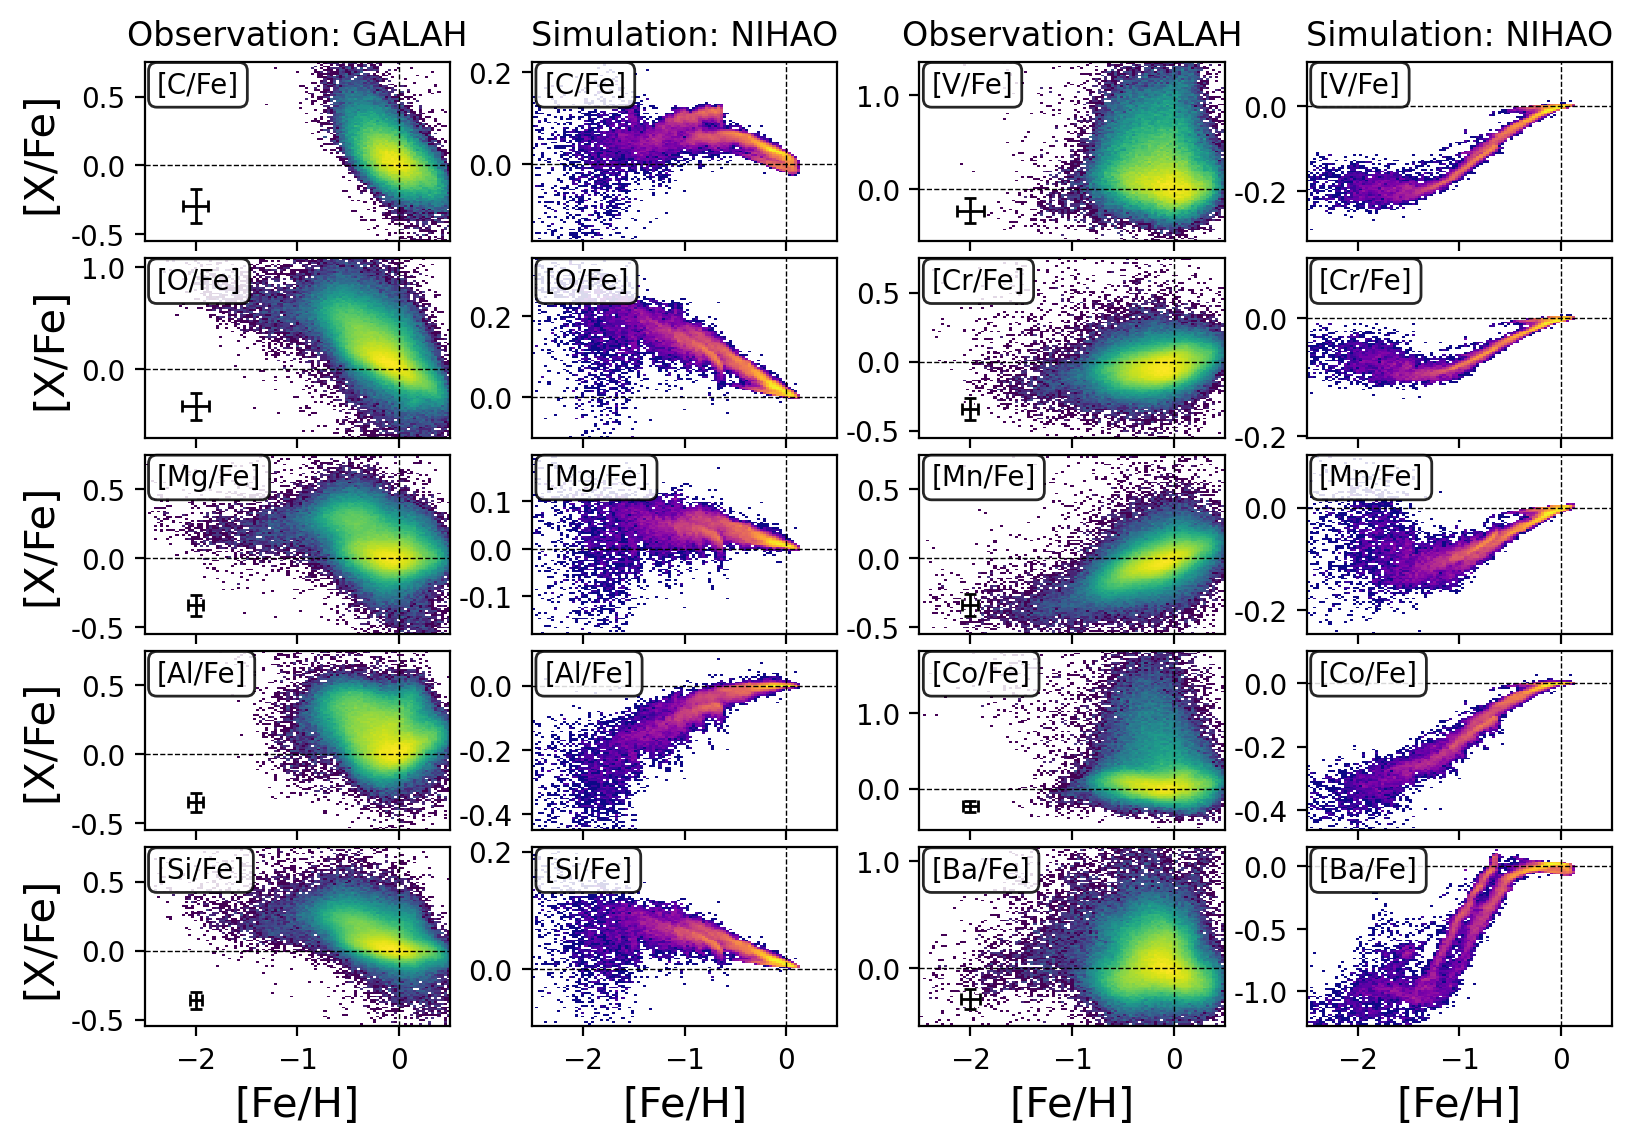
\includegraphics[width=\textwidth]{figures/Overview_FeH_XFe_Obs_Sim.png}
    \caption{
    \textbf{Distribution of elemental abundances [X/Fe] versus [Fe/H] for the ten elements overlapping between GALAH and NIHAO.} 
    \textbf{First and third rows} show observed data from GALAH and \textbf{second and fourth rows} show the simulated data for the same abundance ratios. Color maps are showing the logarithmic density distributions with brightest colors indicating highest densities. For better visibility, plot ranges are adjusted to the data rather than to be equal among each panel. Dashed lines indicate Solar values.}
    \label{fig:allvsFeH}
\end{figure*}

\SB{Question to discuss: Should we renormalise the [X/H] for the elements so that the solar neighborhood lands at 0, as would be custom by definition?}

\subsection{Aims of Study} 

The main aim of this project is to identify the most suitable plot for identifying accreted structures in the Milky Way. This assessment will be based on our ability to observe clear spectral patterns and trends, as well as the clarity of the plots: quantifying the distinction between populations with Gaussian methods. Based on our understanding of how the elements themselves are produced, we can recognise abundance patterns that are different to those that would be produced through the evolution of the Milky Way and thus must be accreted. We assess a range of elements for this purpose, as there is observed overlap between in situ and accreted abundances of some elements, for example Fe.  Analysing the cosmological simulations will assist in this determination, in confirming the origin of the accreted stars selected via chemical tagging, and thus confirming the methodology.

An improved understanding of accretion within the Milky Way encompasses more accurate stellar ages \citep{Das2020}, merger history \citep{Naidu2020}, stellar formation history and chemical enrichment \citep{DeSilva2015}: all facets which contribute to a more accurate picture of our early Universe and its origins. We are entering an exciting period in the field of galactic archaeology and with more and more increasingly accurate data coming out, we are facing the possibility of unprecedented understanding of the Milky Way’s, and the Universe’s, long and complex history.

%%%%%%%%%%%%%%%%%%%%%%%%%%%%%%%%%%%%%%%%%%%%%%%%%%

\section{Diagnostic plots with simulated data}
\label{sec:comparison}

In Sec.~\ref{sec:intro}, we have identified several observation-based plots that have been used to identify accreted stars in the Milky Way. In this section, we are now concerned with replicating these plots for the simulated Milky Way analogue to first order\footnote{\SB{Come back to this if we figure out that we actually do have to limit the simulation space to the Solar neighborhood - which we have not done yet!}}. For this particular study, we will limit ourselves to the following plots: a) [Fe/H] vs. [Mg/Fe] \citep{Nissen2010}, [Al/Fe] vs. [Mg/Mn] \citep{Hawkins2015, Das2020}, 


Through reading the relevant literature, a clear starting place for data analysis arose: replicating observation-based plots that had demonstrated clear results.  

\begin{figure*}
	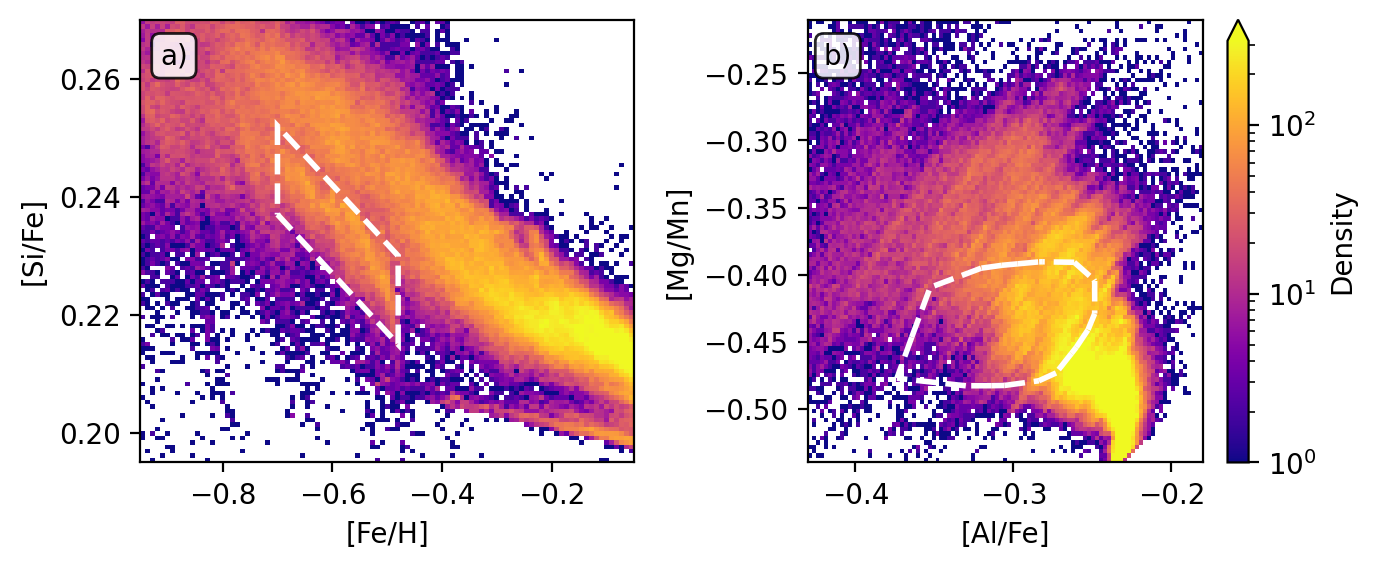
\includegraphics[width=\textwidth]{figures/low_alpha_halo.png}
    \caption{
    \textbf{Chemical abundances for all particles of the simulation (color-coded by logarithmic density) and a subset of particles (selected via white polygon in left plot).} 
    \textbf{Panel a):} iron vs. silicon abundances as tracers of contribution from SNIa and SNII. \textbf{Panel b):} abundance combination [Al/Fe] vs. [Mg/Mn] used to trace accreted stars in observations. A convex hull is used to plot the area of the stars selected via a polygon in panel a).
}
    \label{fig:low_alpha_halo}
\end{figure*}

These plots didn't return the expected results (as explained in detail in Section \ref{sec:obs_vs_sim}), so a range of other plots, of different chemical abundance planes, were produced. \citet{Hawkins2015} outlined the four most suitable combinations to be [$\alpha/Fe$], [C+N/Fe], [Al/Fe], [Mg/Mn]. This informed the next plots made, shown in Figure \ref{fig:alpha}. Although the majority of plots throughout this report are produced on identical axes for clear comparison, the observation and simulation plots were on such different scales that the axes range had to be altered to allow for detail in the plots to be seen clearly. Again, these plots did not return any usable results (see Section \ref{sec:obs_vs_sim}) and so plots of elements over time were produced instead. 
 
 The first step in creating these plots was to align the 'age' data in both datasets, as the simulation data uses time since formation (where a 3Gyr star would be placed at a value of 'tform' = $\sim$ 11Gyr) and the observation data uses stellar age directly. This is a simple matter of subtracting one dataset from 13.8Gyr, but is an important step nonetheless. For this report, the simulation 'tform' column was subtracted from 13.8Gyr to ensure that both datasets being compared could be considered in terms of stellar age.  
Once this had been done, each element (in a ratio with Fe) was plotted over time, in both simulation and observation as shown in Fig.~\ref{fig:BaFetime} for [Ba/Fe]. The elements were tested with a range of elemental abundances, and it was found that the combination of [X/H] produced the most distinct results. This plot then formed the basis of the preceeding steps taken to quantify the separation between accreted and in situ stars, as described more thoroughly in \ref{subsec:quant}.  
 
 All the plots described thus far have been two dimensional histograms, with a colourscale to represent density. Because of the high volume of stars we are working with, the colourscale is logarithmic-based. These were chosen as the clearest representation of the data, as they most clearly highlight overdensities through distinction in colour, as well as the various trends and shapes that are apparent in the substructure.  
 Essentially, the first step of this project was to create a number of abundance planes, based on the literature, and explore a large range of elemental combinations, subsets, and types of plots. When these were found to provide little clarity, elements were plotted over time instead, which form the basis of this report's \hyperref[sec:discussion]{discussion}, recommendations and conclusions.
 
 
 \subsection{Quantifying Results}
\label{subsec:quant}
This project relies on comparison between plots- comparing between elements, observation and simulation, and plots themselves. Whilst an important component of this is visual comparison of the plots, it is also necessary to find a way to quantify the differences between plots. The basis of this quantitative analysis is the assumption that the measurement uncertainties of the observational data are distributed in a Gaussian shape. In essence therefore, the difference between plots will be quantified through the mean of the Gaussian spread $\mu$ and the standard deviation $\sigma$. These values are shown in Figure \ref{fig:hist_labels}, where a discrete, one-dimensional histogram has been plotted and produces two distinct Gaussians, with the corresponding values shown. 
\begin{figure}
	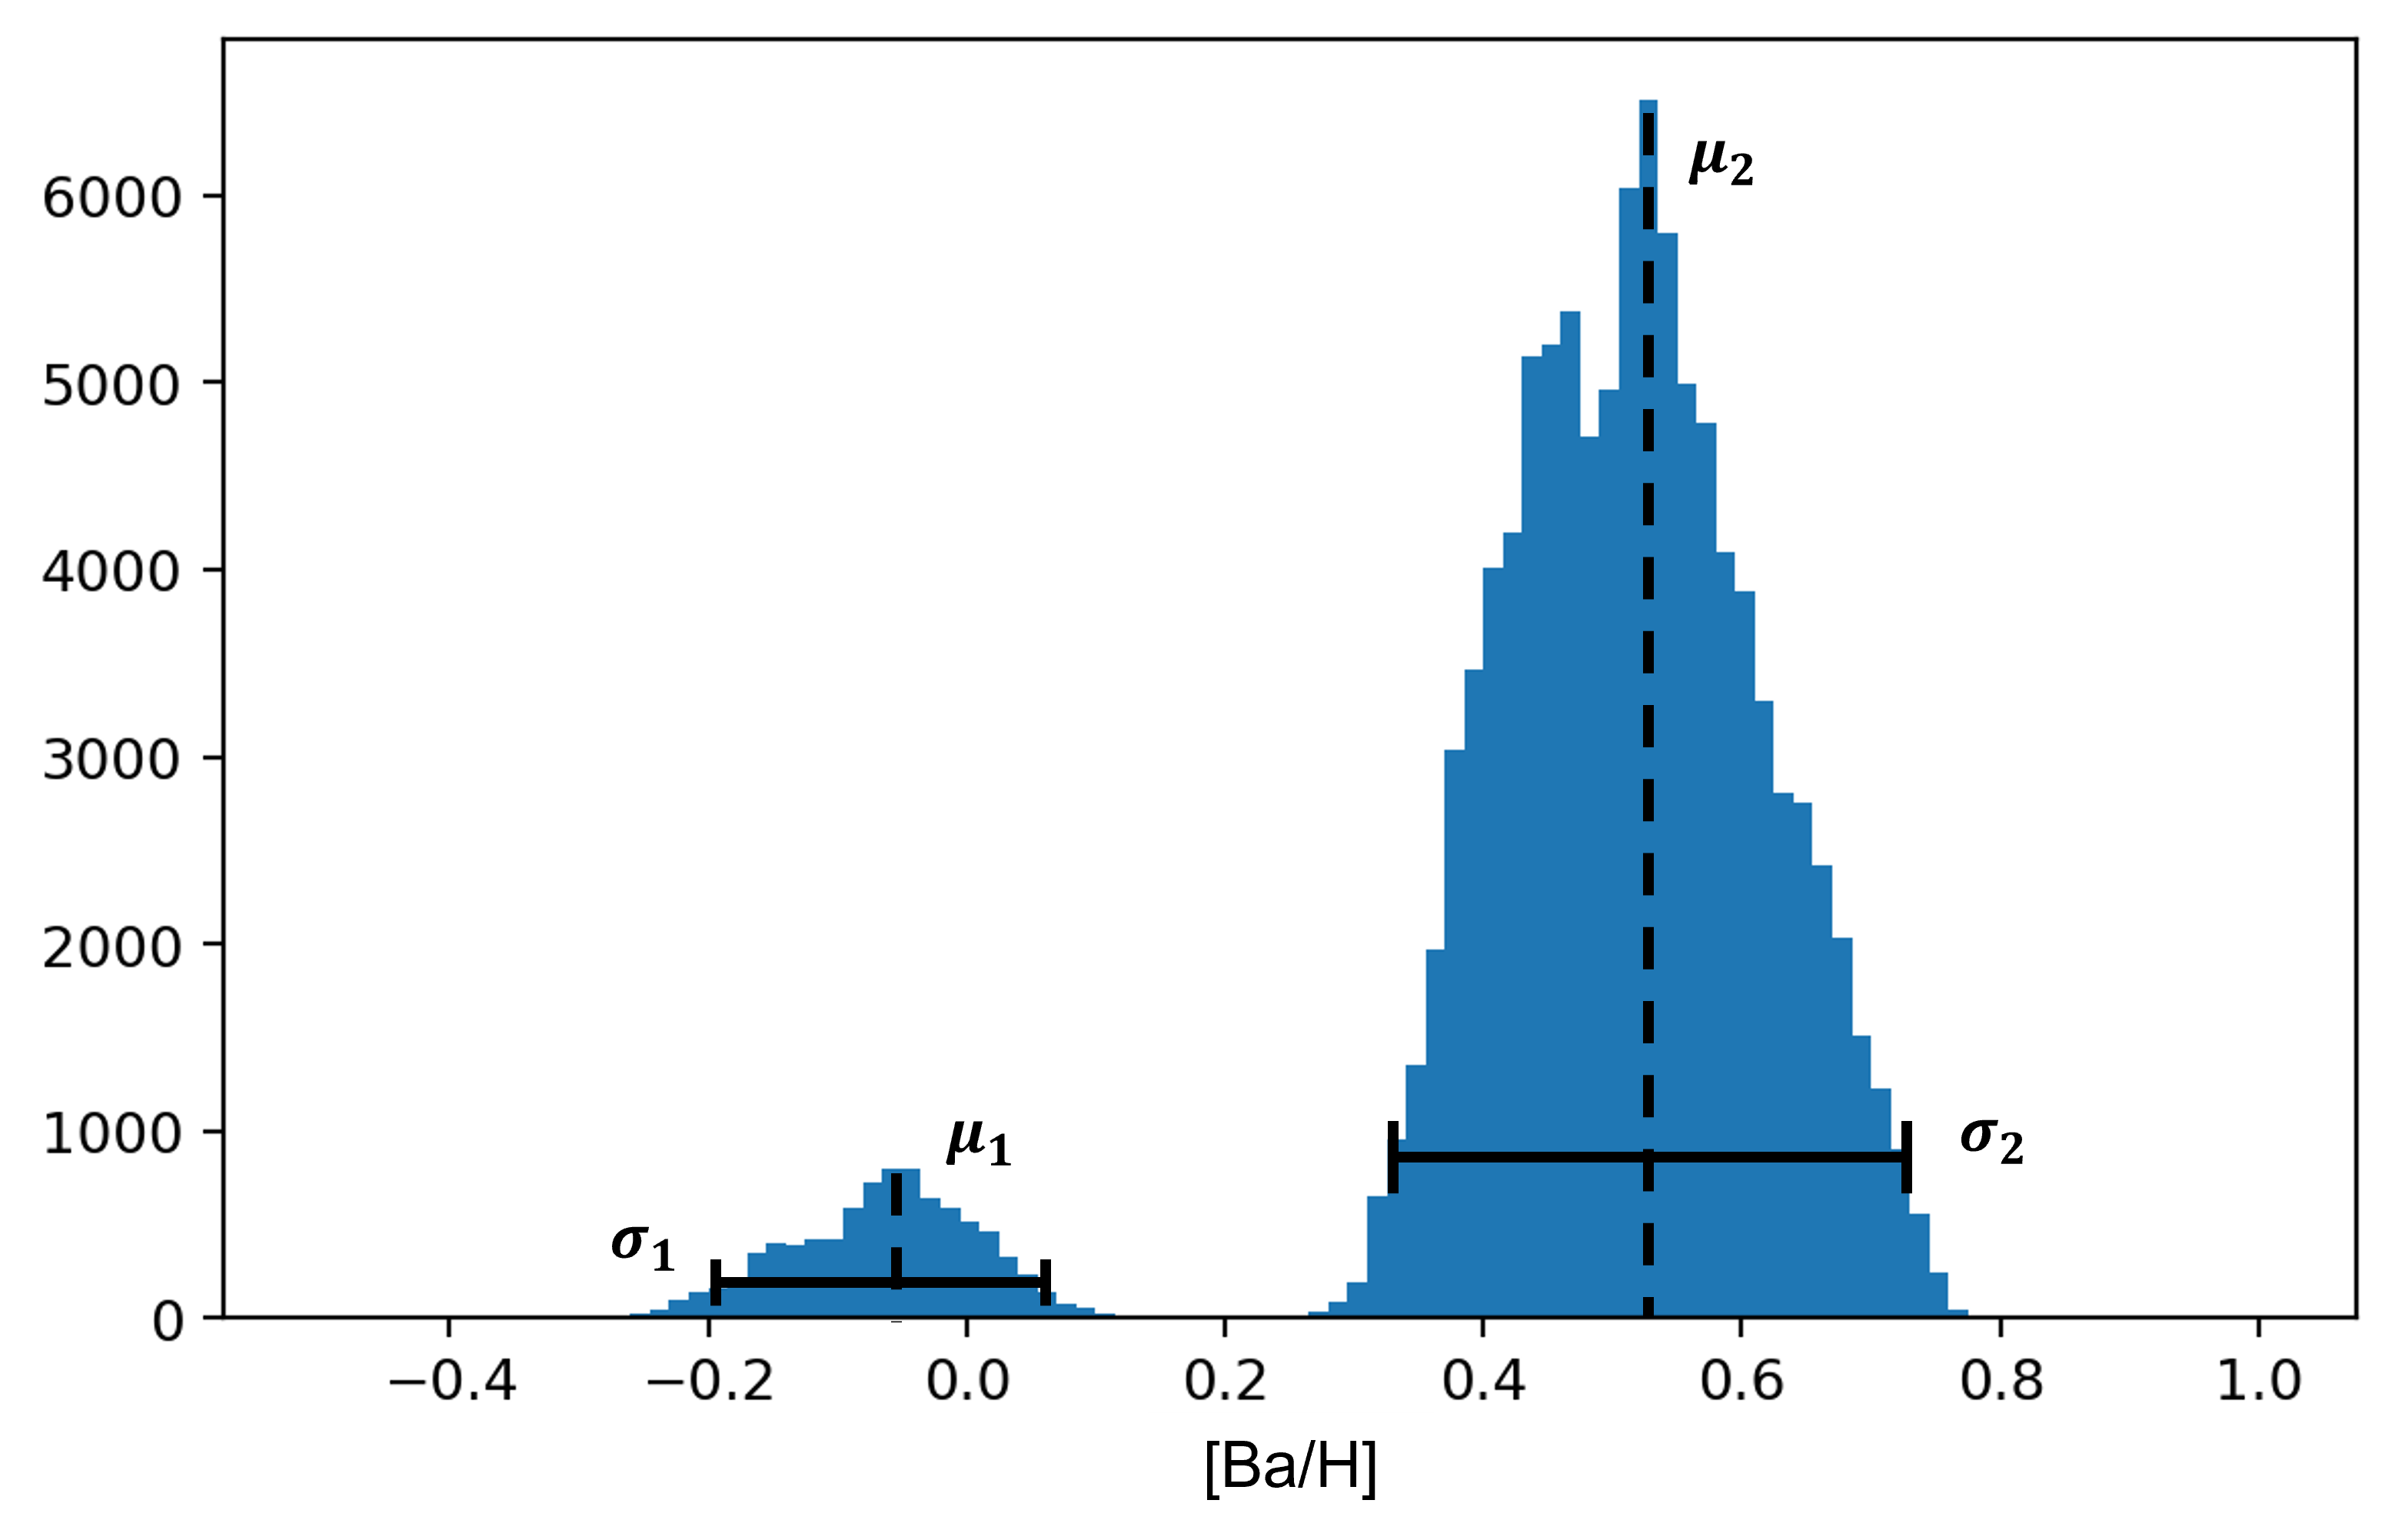
\includegraphics[width=\columnwidth]{figures/hist_labelled.png}
    \caption{A discrete 1D histogram of Barium (used just as an example), with two distinct Gaussian distributions representative of the accreted and in situ populations. This plot has been labelled with diagramatic indicators of the values of mean ($\mu_1$ and $\mu_2$) and standard deviation ($\sigma_1$ and $\sigma_2$) which are used in this project to quantify the separation between populations.}
    \label{fig:hist_labels}
\end{figure}

 
To identify accreted stars, one must be able to identify separate bodies of stellar populations in the data with enough confidence to definitely say they are distinct. This confidence comes from low enough uncertainty in the data to reduce potential overlap between the bodies. \citet{Lindegren2013} produced a research note exploring this exact problem, and specifying an upper limit to the uncertainty possible in the data to still allow for a clear distinction between two bodies of stars. The precision of the data depends on two factors: the separation between the bodies (intrinsic scatter) and measurement uncertainties (extrinsic scatter). 


% Visually, this is made very clear in Figure \ref{fig:lineartime}, where the elemental ratio of Barium over Hydrogen has been plotted over time and there are two distinct streams of stars, as highlighted with different colours. Linear equations to assist in the quantification have been fitted to the two curves in 1Gyr increments, symbolised by the alternating shades of the two colours.  This figure makes the two different stellar bodies (accreted and in situ) that we are trying to distinguish between very clear, however the next crucial step is to be able to quantify the separation between the two. To do this we can compare the linear plots of each Gyr increment: finding the mean value ($\mu$) of the line, and the standard deviation ($\sigma$) of the scatter. An estimate of these values can be made easily through a one dimensional histogram of the data (see Figure \ref{fig:hist}, wherein there are two clear Gaussian distributions visible, and the values of ($\mu$) and ($\sigma$) can be estimated by sight for now, before being used in accordance with Equation \ref{eq: sep} to calculate the separation. The accurate calculation of these values will be done through Python in the coming weeks.  

% \begin{figure}
%     \includegraphics[width=\columnwidth]{SIM Ba over time acc vs situ.png}
%     \caption{The elemental component of Barium over time from the cosmological simulations, with two distinct streams. A linear line has been fitted to 1Gyr increments (shown as alternating shades of the same colour). The brown curve represents the in situ stars and the pink curve represents accreted stars, segmented  into linear chunks.}
%     \label{fig:lineartime}
% \end{figure}

% \begin{figure}
% 	\includegraphics[width=\columnwidth]{histogram.png}
%     \caption{A one dimensional histogram of the same data plotted in Figure \ref{fig:lineartime}, which shows two clear Gaussian distributions among the data, representative of the two stellar bodies in question. This histogram has been limited to all of the stars existent between 4 and 5 Gyrs, for direct comparison between the two linear lines produced above.} 
%     \label{fig:hist}
% \end{figure}

Adapted from \citet{Lindegren2013}, Equation \ref{eq: sep} will be used to quantify this separation. In the case of the simulation data, as this example is, there are no measurement uncertainties which means the standard deviation only depends on the intrinsic scatter of the data. 

\begin{equation} \label{eq: sep}
r = \frac{|\mu_1 - \mu_2|}{\sqrt{\sigma_1^2 + \sigma_2^2}}
\end{equation}

Within this equation, subscripts 1 and 2 represent the two populations in question, as shown in Figure \ref{fig:hist_labels}. To determine the exact numerical values of these quantities, the dataset of each element had to be split into two parts, encompassing the lower and higher Gaussians respectively (1 and 2). \SB{Need to make this more quantitative via Python: This was done visually, through looking at the histogram of each element as in Figure \ref{fig:hist_labels} and setting an upper and lower limit for each sequence.} 



 The process of calculating the r-value using Equation \ref{eq: sep} was performed for each element to determine the most suitable choice for identifying accreted stars. Simply, the element with the highest corresponding r-value will be the plot that we can be most confident in our identification of accreted and in situ stars. The results of these calculations can be found in Table \ref{table: 1}. 


%%%%%%%%%%%%%%%%%%%%%%%%%%%%%%%%%%%%%%%%%%%%%%%%%%
\section{Observation vs. Simulation}
\label{sec:obs_vs_sim}
%%%%%%%%%%%%%%%%%%%%%%%%%%%%%%%%%%%%%%%%%%%%%%%%%%
The first plots produced and analysed were [X/Fe] against [Fe/H], from both the observation and simulation data, which allowed for a side-by-side comparison to be made. [Fe/H] is generally representative of the metallicity of a star, which has significant implications for its age and the ISM from which it was born, which is why [Fe/H] is used often as a basis over which to plot a range of elemental abundances \citep{Buder2022}.  
This abundance plane has been plotted many times throughout the existing literature and has consistently produced a clear distinction in substructure from measured spectra \citep{Das2020, Nissen2010}. When these plots were reproduced for this report, as in Figure \ref{fig:allvsFeH}, in the observation-based plots (right), there are clear overdensities observed, separate to the main, in situ population. When compared to the simulations (left) however, there is very little distinct substructure to be noted. There is significant overlap in the chemical abundance planes in the simulation data, resulting in no clear substructure and making it impossible to identify in situ or accreted stars from the plots.  
One of the key advantages to using simulations is the complete lack of corresponding measurement uncertainties. We would expect the substructure to appear even more clearly in the simulations than in the observations, and the fact that this isn't the case indicates a larger problem in the process. 
\begin{figure*}
	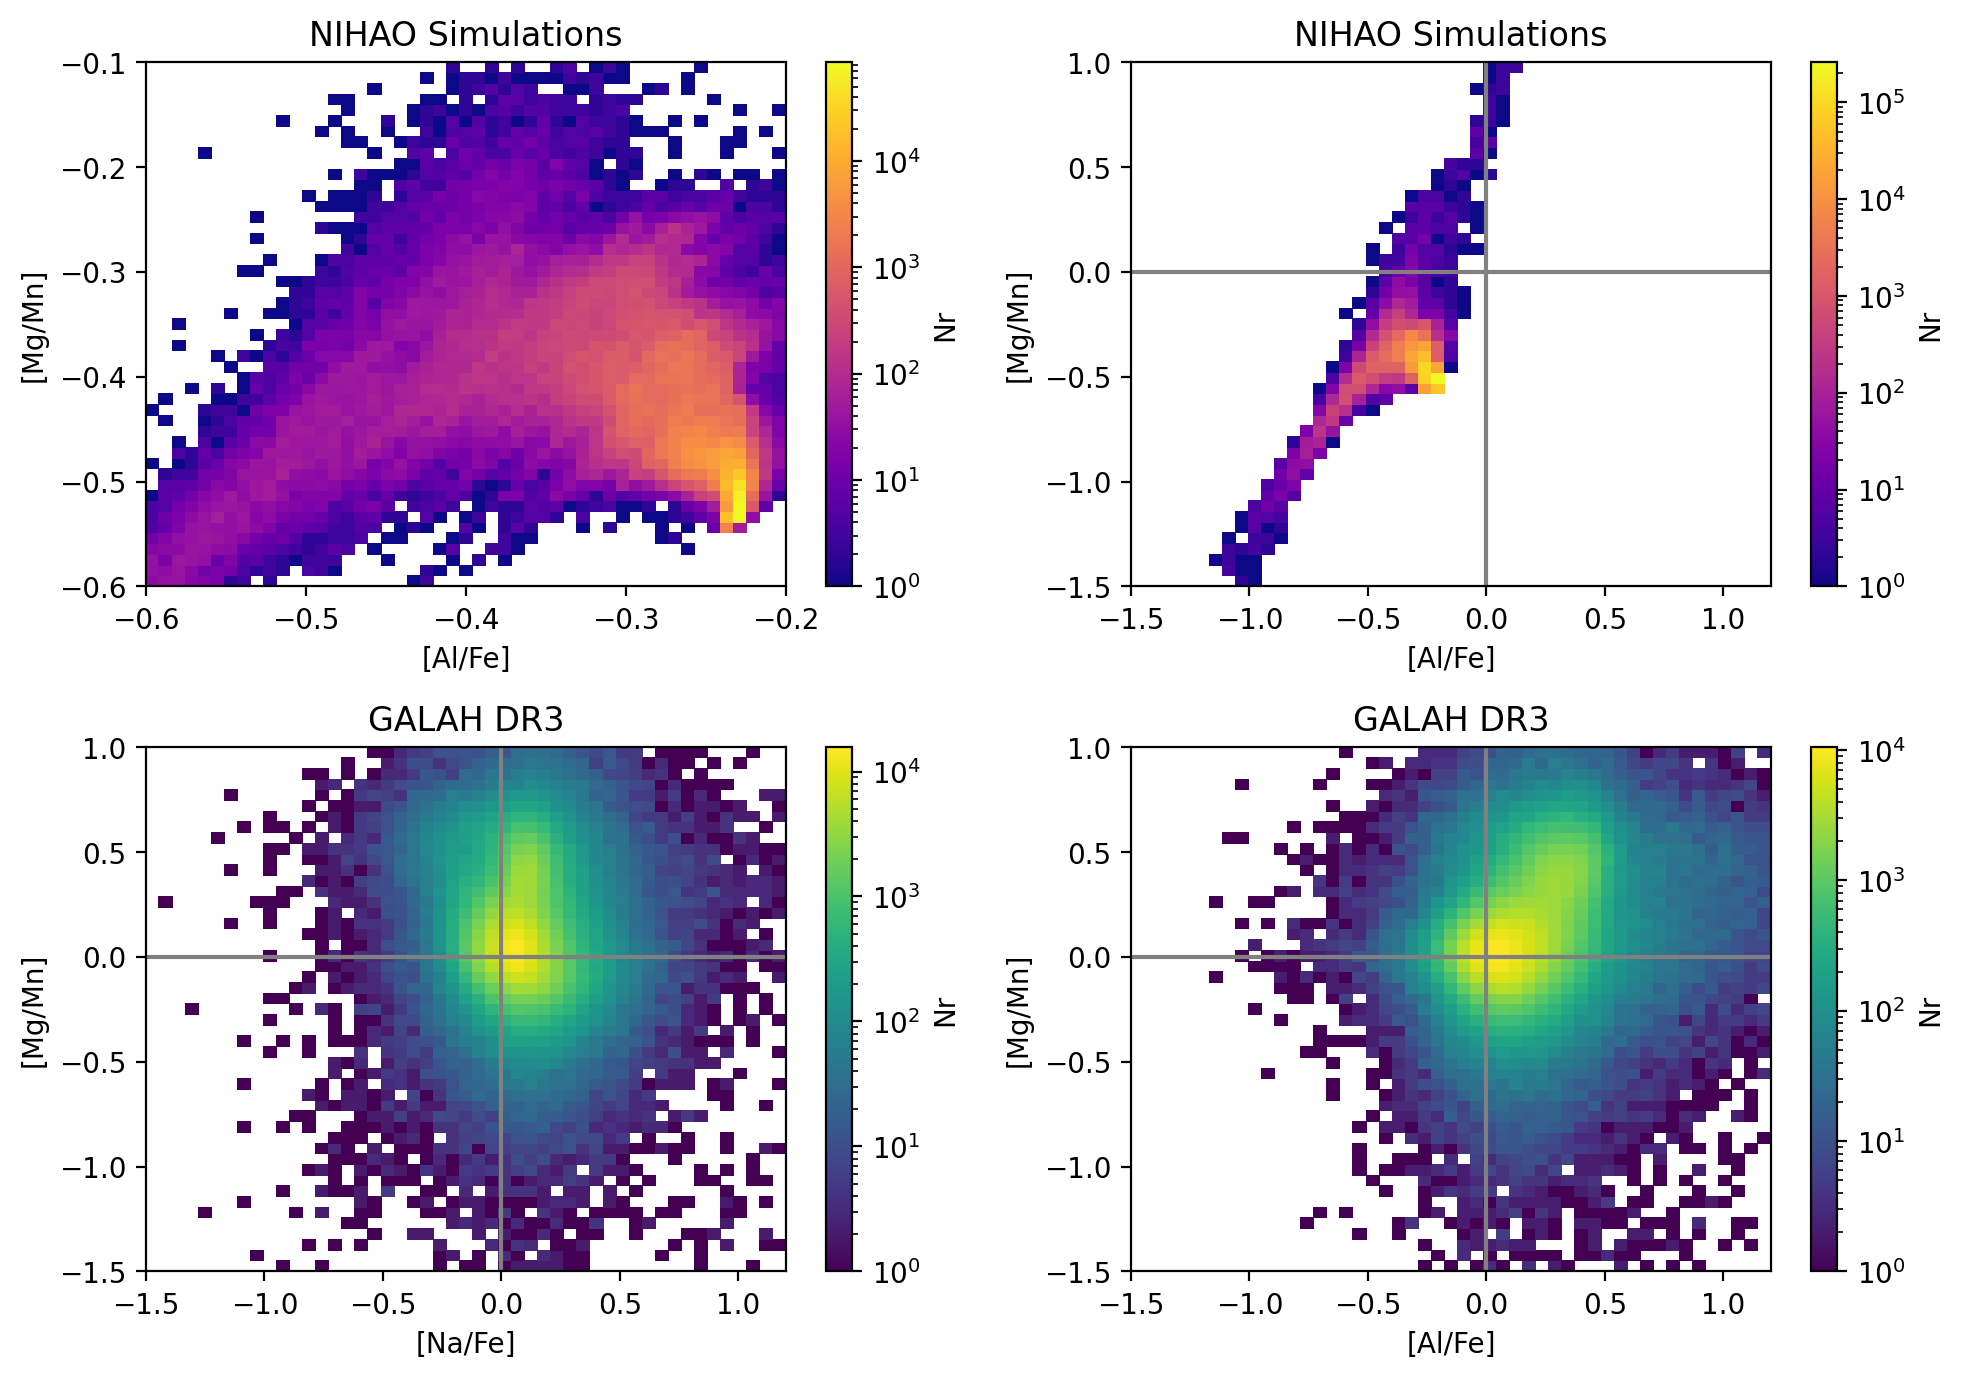
\includegraphics[width=\textwidth]{figures/[MgMn] vs [AlFe].png}
    \caption{Simulation (left) vs observation (right) of alpha element Mg against Mn, plotted over [Al/Fe]. The two plots are on separate axes as the observational plot had to be zoomed in significantly to show any sufficient detail. The zeropoints are completely different, with the axes representing the solar abundances at [0,0] not visible on the observational plot.}
    \label{fig:alpha}
\end{figure*}

Having discounted abundance planes of [X/Fe] vs [Fe/H] as a viable option using these particular simulations, the next step was to assess high and low $\alpha$ haloes. The $\alpha$ elements include Mg and Si, and tend to be of lower abundance in accreted stars. These elements were plotted in combinations of [Si/Fe] vs [Fe/H], as seen in Figure \ref{fig:allvsFeH} and [Mg/Mn] vs [Al/Fe]. Analysing these planes using TopCat, as shown in Figure \ref{fig:low_alpha_halo} made it clear that an overdensity in one plane did appear as an overdensity in the second plane. This provided a good indication that $\alpha$ elements would show distinction in more complete plots of the simulated data. These plots are shown in Figure \ref{fig:alpha}, where the abundance plane [Mg/Mn] vs [Al/Fe] is assessed in the hopes of distinguishing high and low alpha stars.  
Once again, despite clear substructure visible in the GALAH plots, there are no distinct stellar populations visible in the simulation plots. It was expected that the high and low alpha haloes, which, as described in Section \ref{sec:intro} represent young and old populations of stars respectively \citep{Das2020}, would be distinguishable in the plots. However, this was not the case in any viable plots of Mg or Si. Once again, there is no substructure visible in the simulation plots and these abundance planes are not deemed suitable for the purposes of this project.  
Based on the unexpectedly indistinct results produced by plotting abundance planes with known substructure, like the low and high alpha haloes, it was deemed futile to continue delving further into attempting to identify the most suitable abundance plane. Instead, this report turns to the question of other observables that could instead be used to diagnose accretion. Chemical abundances alone did not return usable results, so from the range of other information provided by both GALAH and the simulations, the research now turns to the question of chemical evolution- exploring chronological plots to investigate the difference in evolution between accreted and in situ stars.  



% \begin{figure*}
% 	\includegraphics[width=\textwidth]{4 way comp.png}
%     \caption{A quadrant comparison of two subsections of stars in the abundance plane of [Mg/Mn] vs [Al/Fe], selecting metal-poor stars (top) and higher-metalstars (bottom). The two plots on the left are from the simulations and the two on the right are from observations}
%     \label{fig:4waycomp}
% \end{figure*}

% \begin{figure*}
% 	\includegraphics[width=\textwidth]{COMP high low alpha (2).png}
%     \caption{Stars selected in the [Mg/Mn] vs [Al/V] abundance plane, with two different subsets representing the high (lower) and the low (upper) alpha halos. On top of this is the direct comparison between the simulation (left) and the observation (right) data.}
%     \label{fig:highlowalpha}
% \end{figure*}

% \begin{figure*}
% 	\includegraphics[width=\textwidth]{Al against Fe.png}
%     \caption{The abundance plane of [Al/Fe] against metallicity ([Fe/H]), with simulation on the left and observation on the right. This is just one element of the 9 abundance planes that have been plotted and will be included in the research.}
%     \label{fig:AlvsFe}
% \end{figure*}

% Delving deeper, the plots of [Mg/Mn] against [Al/Fe], and [Si/Fe] against [Fe/H] were produced through TopCat and compared, as suggested by \citep{Hawkins2015}. This allowed for a cursory consideration of the limitations of the methods used, through the exploration of subsets and overdensities appearing in distinct abundance planes. This comparative plot is shown in \ref{fig:low_alpha_halo}  
% Then, in accordance with Hawkins \citeyear{Hawkins2015} and Das et al \citeyear{Das2020}, [C+N/Fe] vs. [Fe/H] will be plotted. This will require some more in-depth manipulation of the data; reverse engineering the fits file so that we are able to use data of C+N. Once this has been done however, it will be compared to the plot the authors have produced from observational data. This plot has not yet been created, but I have included an example plot in Figure \ref{fig:C+N/Fe} from \citep{Das2020} to demonstrate what kind of plot we are expecting from this.  

% \begin{figure}
% 	\includegraphics[width=\columnwidth]{Das2020C+N.png}
%     \caption{The plot taken from Das et al \citeyear{Das2020}, that will be compared to the plots produced in this report of the abundance plane [C+N/Fe] vs. [Fe/H]. *** This will be replaced with my own comparative plots when I have made them!}
%     \label{fig:C+N/Fe}
% \end{figure}


% \begin{figure*}
% 	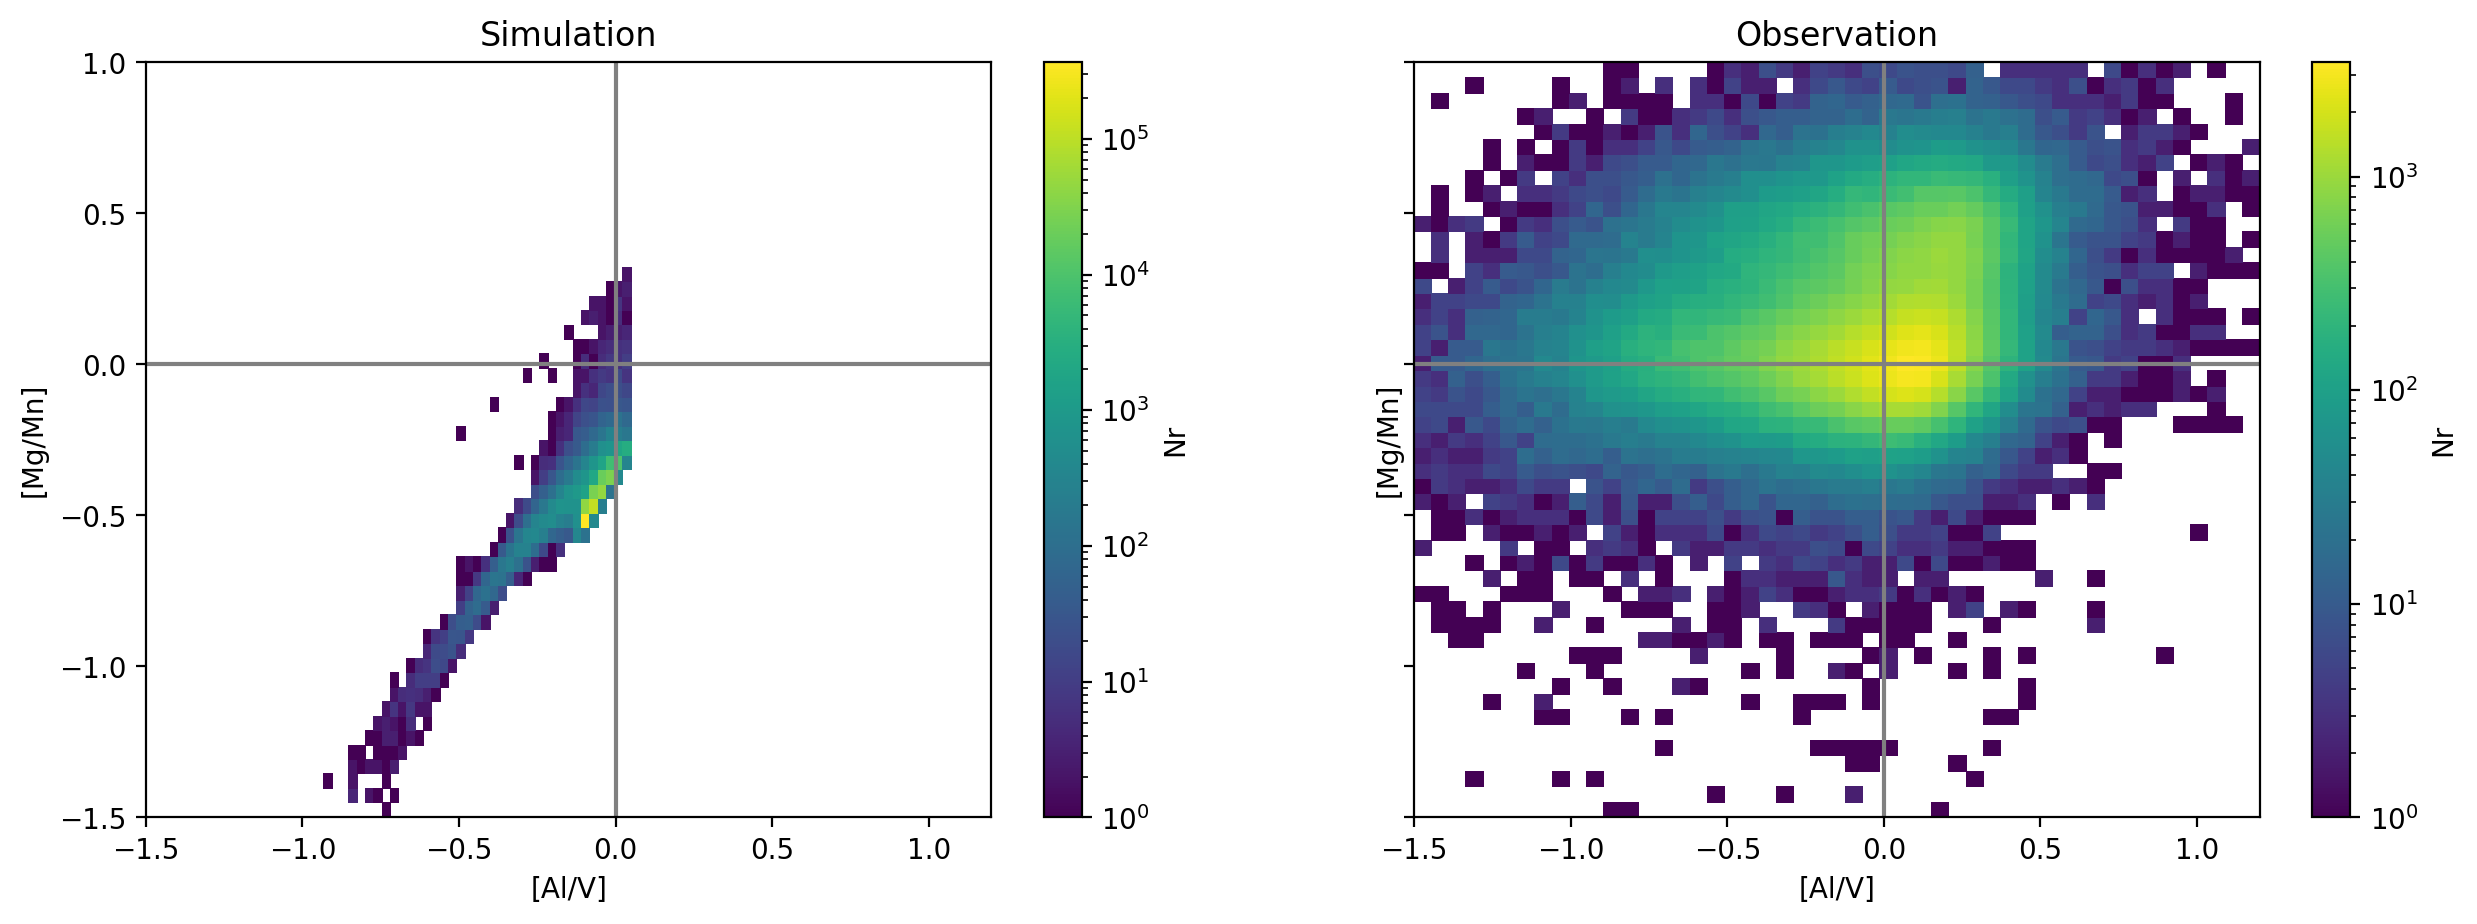
\includegraphics[width=\textwidth]{[MgMn] vs [AlV].png}
%     \caption{The abundance plane of [Mg/Mn] against [Al/V]: a direct comparison of the simulation data (Left) and observational (Right). These plots were created with Figure 4 as the basis}
%     \label{fig:example_figure}
% \end{figure*}



% Amongst the plots created to isolate the separate stellar bodies of in situ and accreted stars are the low and alpha halos (plotted in Figure \ref{fig:highlowalpha}, different subsets of metallicities in Figure \ref{fig:4waycomp} and plotting elements over time as in Figure \ref{fig:lineartime}. The process of finding a precise and quantifiable method of comparison is outlined below, but these plots will all be assessed to determine which one most clearly and with the most statistical confidence highlights two distinct stellar populations. Then, different combinations of elements will be tested to the same end. Equally, these plots will be considered from both the cosmological simulations and the observational data, as below. 


%%%%%%%%%%%%%%%%%%%%%%%%%%%%%%%%%%%%%%%%%%%%%%%%%%
\section{Plots of Chemical Evolution}
\label{sec:evolution}
%%%%%%%%%%%%%%%%%%%%%%%%%%%%%%%%%%%%%%%%%%%%%%%%%%

Elements are created through a variery of pathways and in particular with a time- and environment-dependent manner \citep{Kobayashi2020}. It is clear therefore that chemical enrichment is intrinsically linked to stellar age, most crucially because chemical abundances remain unchanged from birth. This means that plotting elemental abundances over time should produce clarity between accreted and in situ stars, as there should be clear patterns in how the elements evolved over time.  And in this simulation plot, finally there are distinct stellar populations, represented by two 'streams'. The upper stream in these plots is representative of the in situ population of stars, and the lower, the accreted population. This explains the similarly shaped path of evolution that both follow, but accreted populations tend to join the Milky Way from smaller galaxies with less massive stars. This means that the stars are less metal-heavy and will therefore have a generally lower component of elemental abundance in their evolution, as is shown.  

The simulation plots are very clear- which is not reflected in the observational plots. The reason for this is the statistically massive measurement uncertainties that correspond with age measurements. As explained in Section \ref{sec:intro}, stellar ages are estimated using isochrone fitting and are very reliant on probability, with measurement uncertainties of around $30-50\%$ of the age in question. These uncertainties are responsible for the copious scatter seen in the observational plots, and means that with our current ability to estimate stellar ages, it is impossible to see distinct substructure. With less uncertainty (such as the simulation plots) distinct populations become clear, which provides clear motivation for further investigation into these plots as diagnostic tools. 
\begin{figure}
	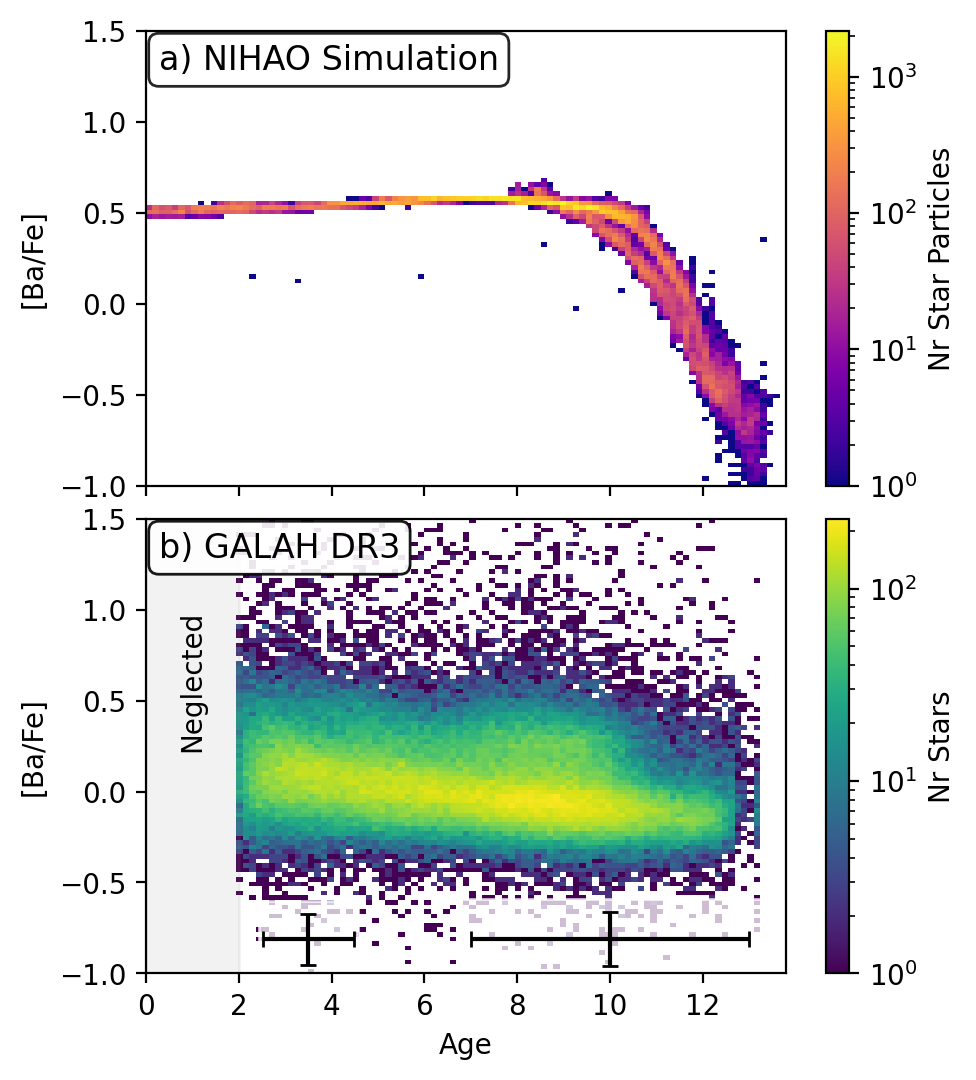
\includegraphics[width=\columnwidth]{figures/Ba_Fe_time.png}
    \caption{Barium abundance in a ratio with Iron [Ba/Fe] as a function of age. Simulation data (top) and GALAH data (bottom) shows clear differences in scatter. Although not entirely separate, it is clear that there are two different overdensities in a 'stream'-like shape.}
    \label{fig:BaFetime}
\end{figure}
\begin{figure}
	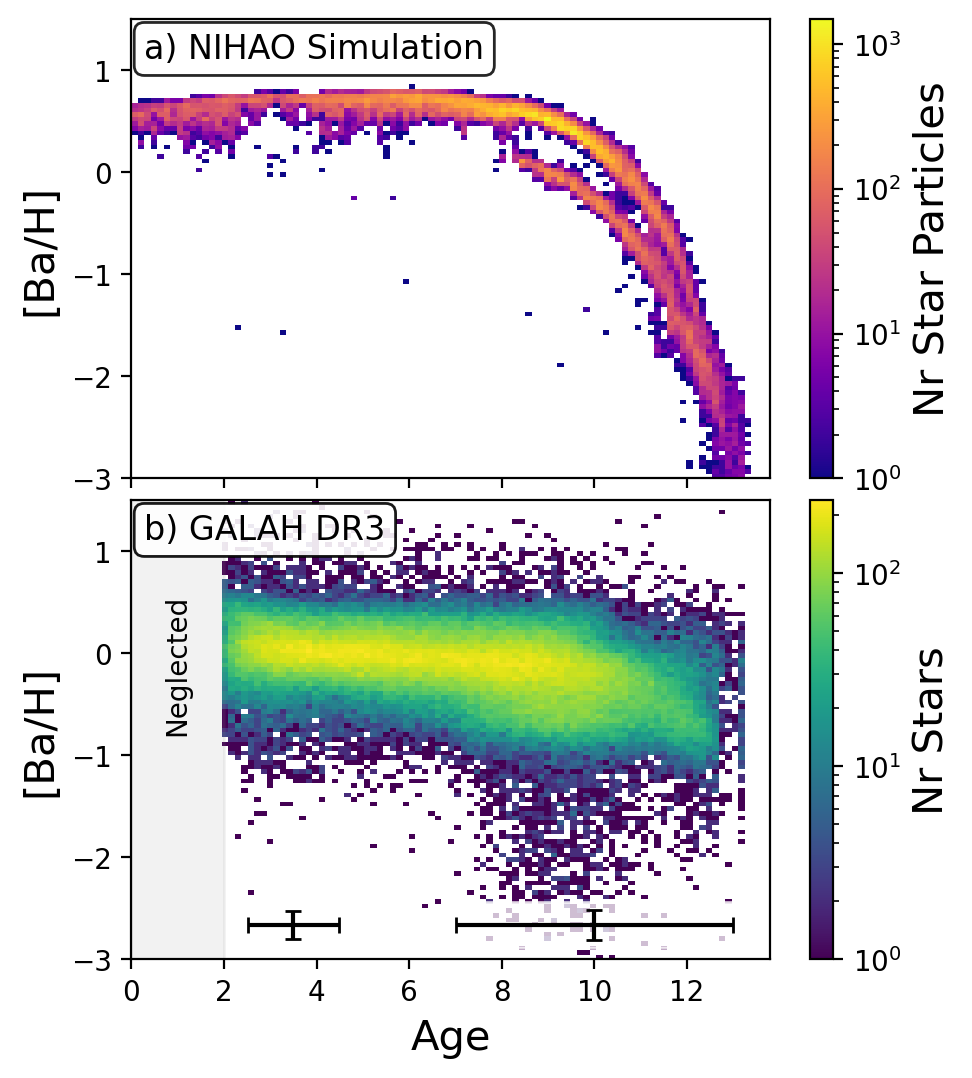
\includegraphics[width=\columnwidth]{figures/Ba_H_time.png}
    \caption{Simulation (top) vs observation (bottom) plots of Barium's evolution with age, with Ba plotted in a ratio against H instead of Fe. The top stream represents the in situ stars, while the lower stream is stars that have since accreted and hence follow a similar evolution path but at lower element abundances.}
    \label{fig:BaHtime}
\end{figure}


Figure \ref{fig:BaHtime} shows the elemental ratio of [Ba/Fe] over time. This same plot was created using every elemental combination available in the dataset, and it was found that the combination of [X/H] over time produced the clearest plot, as in Figure \ref{fig:BaHtime}. Hydrogen, being formed in the Big Bang nucleosynthesis, is not enhanced or affected by time, whereas metals like Fe are. This is why [X/H] plots are decidedly clearer than [X/Fe], as Fe is being simultaneously enriched along with Ba. 

\begin{center}
\begin{table}
    %\caption{One dimensional histograms of each element, used to determine an upper and lower limit so that t}
    \centering
    \begin{tabular}{ |c|c| } 
         \hline
         Element & {Discrete r-value} \\ 
         \hline\hline
          Mg & 6.1  \\ 
         \hline
         C & 5.3  \\ 
         \hline
         Mn & 5.7 \\
        \hline
         Si & 6.0 \\
         \hline
         Ba & 4.6 \\
         \hline
         V & 6.1 \\
         \hline
         Co & 6.4 \\
         \hline
         Al & 6.3 \\
         \hline
         Cr & 5.9 \\
         \hline
         O & 6.0 \\
         \hline
    \end{tabular}
    \caption{The calculated r-values (for separation significance) for each element available in both datasets}
    \label{table: 1}
\end{table}
\end{center}

To determine the element (X), that would be the most suitable option for these plots, the r-value of each element was calculated. The full process of this calculation is described in Section \ref{subsec:quant}, and the results are tabulated below. 



The results make it clear that Cobalt has the highest r-value and therefore should produce the clearest plots. However, there is a relatively marginal difference between all elements, particularly the top few, and so these results do not indicate that Co is the only viable element for this purpose. The small margin between elements in separation significance implies that there is need for further consideration of other variables, such as our ability to recognise the elements in spectral lines.  
The ability to recognise spectral lines is a complex issue with a number of contributors, but for the purposes of this report, one simple way of quantifying this is through mean uncertainty. Table \ref{table: 2} shows each element with its corresponding mean uncertainties calculated. 
%The reason for including the number of measurements is that if measurements couldn't be taken of an element because the spectra wasn't clear enough, this is important to know. C has a very low number of measurements taken which, on top of the high uncertainty, further disqualifies it as a good candidate. 
From this table, it is clear that Co has quite a high average measurement error and thus, despite displaying the largest separation significance, would not be the most suitable element to use. Combining the results of Tables \ref{table: 1} and \ref{table: 2} leads to a preliminary conclusion that Al would be one of the most recommendable elements to use for diagnostic purposes, due to its large number of measurements, and corresponding low uncertainty.  
\begin{center}
\begin{table}
    \centering
    \begin{tabular}{ |c|c| } 
     \hline
     Element & {Average Uncertainty} \\ 
     \hline\hline
      Mg & 0.11  \\ 
     \hline
     C & 0.15  \\ 
     \hline
     Mn & 0.11 \\
    \hline
     Si & 0.07 \\
     \hline
     Ba & 0.12 \\
     \hline
     V & 0.15 \\
     \hline
     Co & 0.15 \\
     \hline
     Al & 0.08 \\
     \hline
     Cr & 0.10 \\
     \hline
     O & 0.15\\
     \hline
    \end{tabular}
    \caption{Each element with its corresponding \textit{average} measurement uncertainty, based on the GALAH data.}
    \label{table: 2}
\end{table}
\end{center}

% \begin{center}
% \begin{tabular}{ |c|c|c| } 
%  \hline
%  Element & {Number of Measurements} & {Average Uncertainty} \\ 
%  \hline\hline
%   Mg & 504056 & 0.11  \\ 
%  \hline
%  C & 293907 & 0.15  \\ 
%  \hline
%  Mn & 515032 & 0.11 \\
% \hline
%  Si & 515027 & 0.07 \\
%  \hline
%  Ba & 527080 & 0.12 \\
%  \hline
%  V & 243784 & 0.15 \\
%  \hline
%  Co & 408981 & 0.15 \\
%  \hline
%  Al & 522895 & 0.08 \\
%  \hline
%  Cr & 507932 & 0.10 \\
%  \hline
%  O & 519276 & 0.15\\
%  \hline
% \end{tabular}
% %\caption{Table to test captions and labels}
% \label{table: 2}
% \end{center}

The value of r is in units of standard deviation, which means that a separation with r=1 ensures 68\% statistical confidence in the distinct populations being accurate. In turn, if r=2, we can be 95\% confident.
This calculation is particularly useful to inform future research in this subset of galactic archaeology, particularly when using this specific simulation. Through the simulations (with no measurement errors), we can determine values of uncertainties that are required in order for results to be presented with either 68\% or 95\% confidence, which is valuable information to wield for those intending to complete the observations in the future.  
Figure \ref{fig:r_v_age} shows each element plotted with r-value against age uncertainty (in Gyr). These particular plots were created using data between 4 and 5 Gyr, which means that a 1 Gyr uncertainty is equivalent to just over 20\%. From these plots, we can see that there is a fair amount of variance between the elements. Regardless, it is clear that at an uncertainty of around 1.25 Gyr (or 25\%) the r-value begins to increase. At the next interval of around 0.75 Gyr (or 15\%) there is a very rapid increase in confidence. This informs us that ideally, we are striving for an uncertainty of less than 15\%, which is significantly lower than the uncertainties we are working with at the moment. 
 

\begin{figure}
	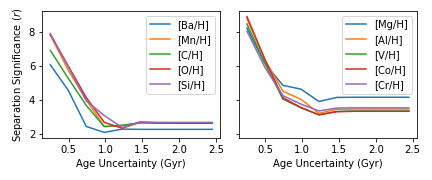
\includegraphics[width=\columnwidth]{figures/same_axis_r_age.png}
    \caption{Separation significance $r$ against age uncertainty (in Gyr) for all elements. These plots were made using data in the time-span between 4 and 5 Gyr after formation. So a 1 Gyr uncertainty is just over 20\% uncertainty. The five elements in the right-side plot have notably higher r-values than those in the left plot. The figure clearly demonstrates the age uncertainty at which we can become quite confident that we are observing two separate populations.}
    \label{fig:r_v_age}
\end{figure}

\begin{figure}
	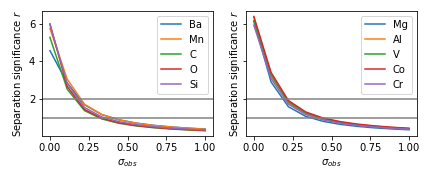
\includegraphics[width=\columnwidth]{figures/same_axis_r_sigma.png}
    \caption{Similar to Figure \ref{fig:r_v_age}, this plot shows all elements on an axis of their separation significance $r$ as a function of measurement noise. There are two horizontal lines at $r=1$ and $r=2$ which show the points at which we can be 68\% and 95\% confident (respectively) that we are observing two distinct populations. It is clear that these values are quite similar for all elements.}
    \label{fig:r_v_obs}
\end{figure}



Similarly, we can plot the separation significance over observation noise, instead of age uncertainty. This will inform the limit of noise that we must be observing below to ensure reliable results, shown in Figure \ref{fig:r_v_obs}. 
To calculate the observational noise ($\sigma_{obs}$), we use Equation \ref{eq:sigma_obs}, which states:
\begin{equation} \label{eq:sigma_obs}
r_{obs} = \frac{|\mu_1 - \mu_2|}{\sqrt{\sigma_1^2 + \sigma_2^2}} = 
\frac{|\mu_1 - \mu_2|}{\sqrt{\sigma_{1,obs}^2 + \sigma_{2,obs}^2}}
\end{equation}
And therefore, that
\begin{equation} \label{eq:sigma_obs_2}
\sigma_{1,obs}^2 = \sqrt{\sigma_1^2+\sigma_{obs}^2} \end{equation}\begin{equation} 
\sigma_{2,obs}^2 = \sqrt{\sigma_2^2+\sigma_{obs}^2}\end{equation}
These equations were used to plot $\sigma_{obs}$ along the x-axis, in units of dex. 

 There is very little range between elements on these plots, and it is clear that all elements require a level of noise to be below approximately 0.4 to be 68\% sure the populations are separate, and below 0.2 to be 95\% confident. Within the accessible GALAH dataset, we can access the corresponding measurement uncertainties, and find that most, but not all, measurements of chemical abundances fall below these thresholds - if they can be measured and are reported. This indicates that uncertainties in ages are a much more impactful barrier to these results. 
  


% \begin{figure}
% 	\includegraphics[width=\columnwidth]{r_vs_noise_Ba_Si.png}
%     \caption{CAPTION}
%     \label{fig:r_vs_noise_Ba_Si}
% \end{figure}

% \begin{figure}
% 	\includegraphics[width=\columnwidth]{r_vs_noise_Mg_Cr.png}
%     \caption{CAPTION}
%     \label{fig:r_vs_noise_Mg_Cr}
% \end{figure}

% Figure \ref{fig:highlowalpha} shows a plot of the stellar bodies of the high alpha and low alpha stellar halos, which is one possible plot that will be useful in the search for large separations. One of the next steps in this research project will be to quantify the separation between these two populations in a variety of chemical abundance planes to find the largest difference. Figure \ref{fig:4waycomp} shows the plots of low-metal and "high"-metal stars, which visually show a significant difference. Again, this will be determined in numbers, repeating the process through a variety of abundance plane combinations to find the most suitable candidate. 




% The separation between populations referred to here is represented in Figure \ref{fig:Gauss_sep}, which highlights how a difference in separation (in standard deviation units) can allow for distinction between the two populations. The top histogram is separated by r=2.0, the bottom by r=2.4. One can clearly see that with the larger separation, two distinct Gaussian populations are clear. 


 

% \begin{figure}
% 	\includegraphics[width=\columnwidth]{Gaussian separations.png}
%     \caption{Plot taken from \citep{Lindegren2013} demonstrating the difference in statistical confidence that the r value (in units of standard deviation) can provide. The top histogram has an r value of 2.0 between the two stellar bodies and it is indistinguishable that there are two separate populations in the Gaussian curve of best fit. The bottom histogram meanwhile, has a separation of 2.4 standard deviations, and it is clear that there are two seperate Gaussian-like shapes in the data, reflecting two separate bodies.}
%     \label{fig:Gauss_sep}
% \end{figure}

% \begin{figure}
% 	\includegraphics[width=\columnwidth]{Nvsr.png}
%     \caption{Plot from \citep{Lindegren2013}, showing the relationship between sample size and standard deviation. It demonstrates that the larger the distinction between the Gaussian distributions, the higher the accuracy can be obtained with a smaller sample size. Separation here refers to the distinction of two separate Gaussians on one axiss shown in the plots above.}
%     \label{fig:nvsr}
% \end{figure}




% \begin{figure*}
% 	\includegraphics[width=\textwidth]{4 way comp.png}
%     \caption{A quadrant comparison of two subsections of stars in the abundance plane of [Mg/Mn] vs [Al/Fe], selecting metal-poor stars (top) and higher-metal stars (bottom). The two plots on the left are from the simulations and the two on the right are from observations.} 
%     \label{fig:4waycomp}
% \end{figure*}


% \begin{figure}
% 	\includegraphics[width=\columnwidth]{rectangles_on_time_Ba.png}
%     \caption{The plot of Barium's elemental abundance over time, with rectangles selecting increasingly large time ranges.} 
%     \label{fig:rectangles}
% \end{figure}


% \begin{figure*}
% 	\includegraphics[width=\textwidth]{(-2 (Fe H) -1.8).png}
%     \caption{In the abundance plane of [Mg/Mn] against [Al/Fe], this figure shows comparison between the simulation (left) and the observational data (right), taking a subset of stars with the lowest metallicity between -2.0 and -1.8.}
%     \label{fig:lowmetal}
% \end{figure*}

% \begin{figure*}
% 	\includegraphics[width=\textwidth]{(-0.8 (Fe H) -0.5).png}
%     \caption{The metallicity subset between -0.8 and -0.5 of the abundance plane [Mg/Mn] against [Al/Fe]. The simulation is on the left and observation is on the right.}
%     \label{fig:highmetal}
% \end{figure*}


%%%%%%%%%%%%%%%%%%%%%%%%%%%%%%%%%%%%%%%%%%%%%%%%%%
\section{Discussion}
\label{sec:discussion}
This project began with the intention of creating a variety of abundance planes and comparing both simulation and observation data to identify substructure within the plots that was representative of accreted stars. Upon doing so, and observing very little clear substructure in the simulation plots, these plots were deemed insufficient to confidently report any results. As discussed in Section \ref{sec:obs_vs_sim}, there are two major advantages to using cosmological simulations. The first of these is that there are no measurement uncertainties to consider, which should produce clear and accurate plots with no doubt of extrinsic scatter. This means that although some distinct populations were seen in the observational plots, the absence of clarity in the simulation-based plots questions that measurement uncertainties are the main difference between observations and simulations.   
Beyond measurement uncertainties, the second key advantage to the cosmological simulations is that the exact, detailed formation history of the simulated galaxy is known. Knowing what merged with the galaxy and when is crucial in identifying accretion, but this is knowledge that we don't possess to a desirable level for the Milky Way in reality. This poses a challenge in how we can use the cosmological simulations, as we have no guarantee that we are simulating the evolution of the Milky Way. It may also contribute to the discrepancies between the simulations and observations. If the simulations are replicating even a slightly different galaxy, this could explain the lack of clear substructure that we can see in observations. We know that the simulations are based on a merger event that occurred 5Gyr after formation, when a galaxy around $10^9 M_{\odot}$ merged with an in situ galaxy of around $10^{10} M_{\odot}$, values that have been estimated to the order of magnitude by multiplying the number of star particles with their average stellar mass for each sequence of the simulation. Although we do not know the exact sizes or times of accretion events in the Milky Way, the GSE is estimated to be between $10^{8.7}$ and $10^{9.85}\,M_{\odot}$ \citep{Helmi2018,Naidu2020}, which highlights a possible discrepancy between the simulations and the observations. Until we have a more exact understanding of the formation history of the Milky Way, we cannot ensure these simulations are accurate, which is an important caveat to keep in mind.   
From this, the focus of the project underwent a shift, looking instead at other observables beyond chemical abundance that could be used and plotted to identify accreted stars. As Section \ref{sec:intro} makes clear, one of the key advantages to chemical tagging is the unchanging nature of stellar chemistry over time, meaning that a star's current chemical make-up is indicative of the time and place that it was born. Therefore, plotting elemental abundance over time was hypothesised as a good indicator of accretion, where separate populations should be clear. This was plotted and analysed in Section \ref{sec:evolution}, and found that indeed there are two clear stellar populations in the simulation data, indicative of accreted and in situ stars, that were not seen in the observational data due to measurement uncertainties.  
Despite this positive outcome, it is still important to address the possibility of intrinsic overlap between accreted and in situ stars. As discussed, there are two clear streams that have been attributed as accreted and in situ, based on the assumption that the accreted stars would have been born in a smaller galaxy with less massive stars and therefore lower element abundances. This clarity occurs because we know the sizes of the two galaxies that merged. Depending on the size of the real merger in the Milky Way, there could be significantly more overlap between the accreted and in situ populations if the merger was more massive. This means that from the abundance-age plots alone, it is harder to tell if the situ stream is completely made up of Milky Way-born stars. 

A further recommendation is that it would be worth putting effort into further analysing Figures \ref{fig:BaHtime}. Despite the massive amount of scatter in the observations, when Ba was plotted in a ratio with H, there appears to be a hint of an overdensity toward the bottom right of the plot, which could indicate an accreted population. Applying the quality cuts provided in the GALAH data had little effect on how clear this overdensity appears. It is beyond the scope of this project, but with better quality cuts, more time and expertise - and better data, this 'hint' could start indicating something that looks more like the simulations, which would further confirm that plots of elements against time are worth pursuing.  
This project was limited by a number of variables, one of which was simply the number of elements that could be analysed. The caveat for an element to be used in this project was that it had to be included in the datasets of both the simulations, and the GALAH survey. This reduced the total number of elements to just ten. Moreover, although there were quite a number of iron-peak elements, the remaining element groups only contained two options, with Ba being the only neutron capture element. This reduced the ability to make in-depth assessments based on element groups, as the sample size was simply not large enough to consider any trends with certainty. To this end, it could be worth pursuing other datasets with a different choice of elements.  
Moreover, I would strongly recommend similar research is performed with other cosmological simulations, preferably with varied chemistry and formation histories. This would enable researchers to observe exactly how different variables in the simulation affect outcomes. 
The main observational limitation to this project was simply measurement uncertainties, particularly in ages. If the errors corresponding to age measurements can be drastically reduced, plotting elements over time has the potential to be a great diagnostic tool for accreted stars. 


%%%%%%%%%%%%%%%%%%%%%%%%%%%%%%%%%%%%%%%%%%%%%%%%%%

%%%%%%%%%%%%%%%%%%%%%%%%%%%%%%%%%%%%%%%%%%%%%%%%%%
\section{Conclusions}
\label{sec:conc}
The aim of this project was to determine the most suitable diagnostic plot for identifying accreted stars in our Milky Way, through comparison of NIHAO-based cosmological simulations and data from the GALAH survey. The major take-aways from this undertaking were that chemical abundance planes of the simulations possess too much intrinsic overlap to be useful to this particular research project. Plotting elemental abundances against age however, proved fruitful, with very distinct streams representing accreted and in situ populations appearing in the simulation data. These clear streams were not apparent in the observation-based plots, as a result of massive uncertainties that come with the probabilistic nature of estimating stellar ages through isochrone fitting.  
In plotting elements over time, using comparisons through Gaussian distributions, Cobalt was found to be the most distinct element to use, as it had a marginally larger separation significance between the two populations than the other elements. When taking into account the ability to measure element abundances, for example in GALAH, Al provided the best compromise of separation and measurement uncertainties. Moreover, the elemental combination with H was found to produce the clearest results: plotting element abundances [X/H] as a function of time. Overall, reducing uncertainties in ages is a difficult task that may take a long time, but as data and techniques continue to improve these values, there is much potential in using plots of elemental abundances over time as a diagnostic tool for accreted stars. 
%%%%%%%%%%%%%%%%%%%%%%%%%%%%%%%%%%%%%%%%%%%%%%%%%%

% The last numbered section should briefly summarise what has been done, and describe
% the final conclusions which the authors draw from their work.


% Accreted stars appear as overdensities in chemical abundance planes because they are merged with the MW as one galaxy Because they usually come from smaller galaxies than MW, we can assume that they have less massive stars and therefore will be lower in metallicity (lower in [Fe/H])     If I can find an overdensity in one plane that doesn’t correspond with anything interesting in the other plane, it means that there must be a lot of similarities with the MW, which is interesting to note as it means that the galaxy that collided with MW had very similar chemical makeup/stellar formation history/age/mass 

% \section*{Acknowledgements}

% The Acknowledgements section is not numbered. Here you can thank helpful
% colleagues, acknowledge funding agencies, telescopes and facilities used etc.
% Try to keep it short.

%%%%%%%%%%%%%%%%%%%%%%%%%%%%%%%%%%%%%%%%%%%%%%%%%%
% \section*{Data Availability}

 
% The inclusion of a Data Availability Statement is a requirement for articles published in MNRAS. Data Availability Statements provide a standardised format for readers to understand the availability of data underlying the research results described in the article. The statement may refer to original data generated in the course of the study or to third-party data analysed in the article. The statement should describe and provide means of access, where possible, by linking to the data or providing the required accession numbers for the relevant databases or DOIs.


% \section{Cosmological Simulations}
% %%%%%%%%%%%%%%%%%%%%%%%%%%%%%%%%%%%%%%%%%%%%%%%%%%

% We will use the simulation described in the paper by \citet{Ratcliffe2021}.

% You can download the simulation from \url{https://datashare.mpcdf.mpg.de/s/unLXJDEaro5mydt}

% And there is an example code to read in the abundances from the simulation in the file \texttt{example.py} within this overleaf.

% But we will go through this in detail in January 2022.



%TO DO BEFORE SUBMISSION 
%%% Hyperlink all figures and section references 
%%% Check figure and equation numbers



%%%%%%%%%%%%%%%%%%%% REFERENCES %%%%%%%%%%%%%%%%%%

% The best way to enter references is to use BibTeX:
\bibliographystyle{mnras}
\bibliography{bib} % if your bibtex file is called example.bib

%%%%%%%%%%%%%%%%%%%%%%%%%%%%%%%%%%%%%%%%%%%%%%%%%%

%%%%%%%%%%%%%%%%% APPENDICES %%%%%%%%%%%%%%%%%%%%%

% \newpage
% \appendix

%%%%%%%%%%%%%%%%%%%%%%%%%%%%%%%%%%%%%%%%%%%%%%%%%%

% Don't change these lines
\bsp	% typesetting comment
\label{lastpage}
\end{document}

% End of mnras_template.tex
